\chapter{Requisitos y casos de uso}
\section{Requisitos candidatos}
\par En primer lugar se identifican los requisitos que se intentarán cumplir con la solución propuesta.
\par Se agrupan los requisitos según estén más orientados al componente WAF o al componente de TLS.
\par Requisitos orientados principalmente al componente WAF:
\begin{enumerate}[\bfseries{}R1. ]
  \item La solución debe poder ejecutarse en un sistema operativo o máquina independiente de la plataforma de la aplicación web con el
    objetivo de garantizar independencia en las tareas de administración y permitir aplicar un modelo RBAC.
  \item La solución debe disponer de un conjunto básico de políticas de auditoría o bloqueo que permitan proteger la aplicación web frente a
    los ataques más comunes.
  \item La plataforma debe permitir implementar parches virtuales frente a ataques conocidos.
  \item La solución debe permitir la elaboración de reglas personalizadas según las necesidades específicas de la plataforma del cliente.
  \item La plataforma debe ser compatible con el modelo de licencias de {\em software libre\cite{softwarelibre}} tipo
    Licencia Pública General de GNU (en adelánte \acrshort{gpl}, de  sus siglas en inglés \acrlong{gpl}) o Licencia Pública General Reducida
    de GNU (en adelánte \acrshort{lgpl}, de  sus siglas en inglés \acrlong{lgpl}).
  \item La plataforma debe generar logs de seguridad exportables a soluciones externas de gestión de información y eventos de seguridad (en
    adelante \acrshort{siem} de sus siglas en inglés, \acrlong{siem}).
\end{enumerate}

\par A continuación se recogen los requisitos asociados al componente de TLS:
\begin{enumerate}[\bfseries{}R1. ]
  \item La solución debe poder participar en la negociación TLS, presentando certificados confiables a los clientes.
  \item La solución deber poder gestionar los certificados presentados a los clientes incluyendo soporte a la extensión \acrshort{SNI} de TLS.
  \item La plataforma debe soportar TLS versión 1.3, HTTP/2 y otros elementos incluidos en las {\em buenas prácticas de TLS\cite{TLSBestPractices}}.
  \item Debe permitir aplicar soluciones de SSL offloading, entre el WAF y los frontales de la plataforma web, o permitir cifrado punto a punto.
    \par En caso de utilizar la funcionalidad de SSL offloading:
      \begin{enumerate}[label=\emph{\alph*})]
        \item Esta opción es recomendable en entornos controlados en los que prima el rendimiento.
        \item Las comunicación entre el WAF y la plataforma web debe permitir tráfico HTTP.
      \end{enumerate}
    \par En caso de cifrado punto a punto:
      \begin{enumerate}[label=\emph{\alph*})]
        \item Esta opción es recomendable en las soluciones en las que prime la seguridad o en aquellos escenarios en los que no se tenga el control de elementos intermedios, como por ejemplo en entornos cloud o multi-datacenter.
        \item Las comunicación entre el WAF y la plataforma web debe permitir tráfico HTTPS.
        \item El WAF debe confiar en la CA que firma los certificados de la plataforma web o, alternativamente, en los certificados hoja.
      \end{enumerate}
\end{enumerate}

\section{Identificación de actores}
\par Se han identificado los siguientes actores.
\begin{itemize}
  \item {\bf Cliente}. Se utiliza este término para referirse al cliente web que consume los servicios HTTP o HTTPS.
  \item {\bf \Gls{Atacante}}. Se trata de un tipo de cliente malintencionado.
  \item {\bf Plataforma web}. Se considera toda la infraestructura necesaria para servir los contenidos web. En esta infraestructura no se incluyen los elementos desarrollados en el presente proyecto.
  \item {\bf Autoridad de certificación} (en adelante \GLS{CA}). Es el elemento encargado de firmar los certificados TLS. El cliente debe confiar en la CA o en los certificados hoja alternativamente. En caso de cifrado punto a punto el WAF deberá confiar en los certificados presentados por la plataforma web.
  \item {\bf Sistema de virtualización o gestión de contenedores}. Es la infrastructura sobre la que se desplegará la solución WAF. Inicialmente se
    considera una solución de gestión de contenedores como \cite{docker}.
\end{itemize}

\section{Casos de uso}
\par Estos son los casos identificados.
\begin{enumerate}
  \item Caso de uso: Petición identificada como legítima de recurso web.
    \begin{itemize}
      \item Actores: Cliente, plataforma web.
      \item Descripción: El cliente realiza una petición web a nuestra solución. Ésta a su vez realiza la petición a la plataforma web. La
        plataforma web envía una respuesta a la plataforma WAF, que a su vez se la entrega al cliente. En este caso de uso se incluyen peticiones
        legítimas y falsos negativos cuando el WAF falla al detectar un ataque.
      \item Diagrama:
        \begin{center}
          \label{fig:CasoUso1}
          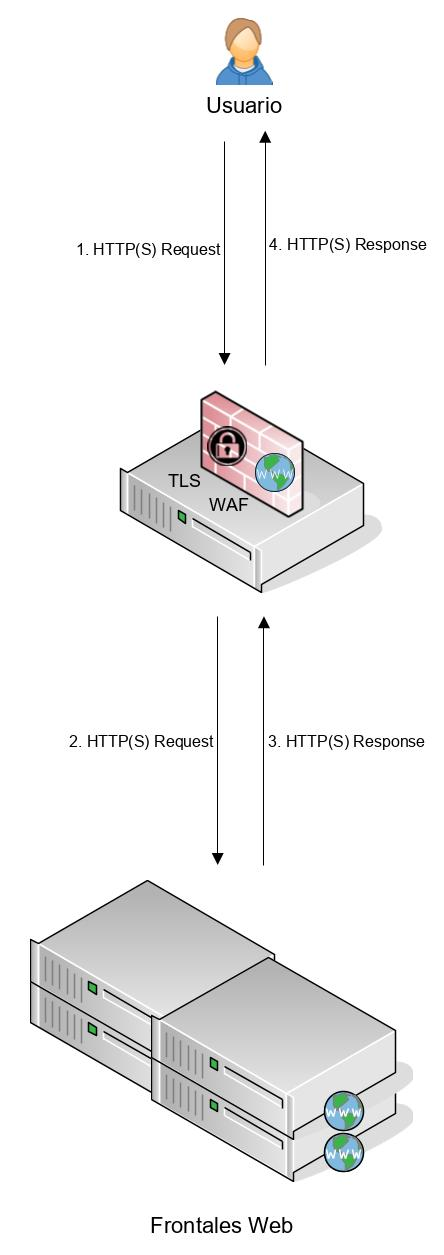
\includegraphics[width=0.4\textwidth]{fig/UseCase1}
        \end{center}
    \end{itemize}
  \item Caso de uso: Petición identificada como no legítima de recurso web.
    \begin{itemize}
      \item Actores: \Gls{Atacante}, plataforma web.
      \item Descripción: El atacante realiza una petición a nuestra solución WAF. El WAF detecta la petición como no legítima y envía un mensaje de
        error al cliente. Este caso de uso incluye ataque reales y falsos positivos cuando se diagnostica como ataque a una petición legítima.
      \item Diagrama:
        \begin{center}
          \label{fig:CasoUsoX}
          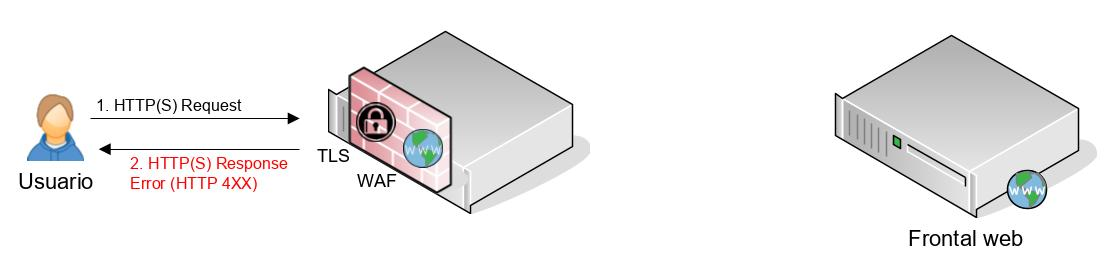
\includegraphics[width=0.4\textwidth]{fig/UseCase2}
        \end{center}
    \end{itemize}
  \item Caso de uso: Petición HTTPS en un entorno con SSL offloading.
    \begin{itemize}
      \item Actores: Cliente, plataforma web.
      \item Descripción: XXXXXXXX
      \item Diagrama:
        \begin{center}
          \label{fig:CasoUsoXX}
          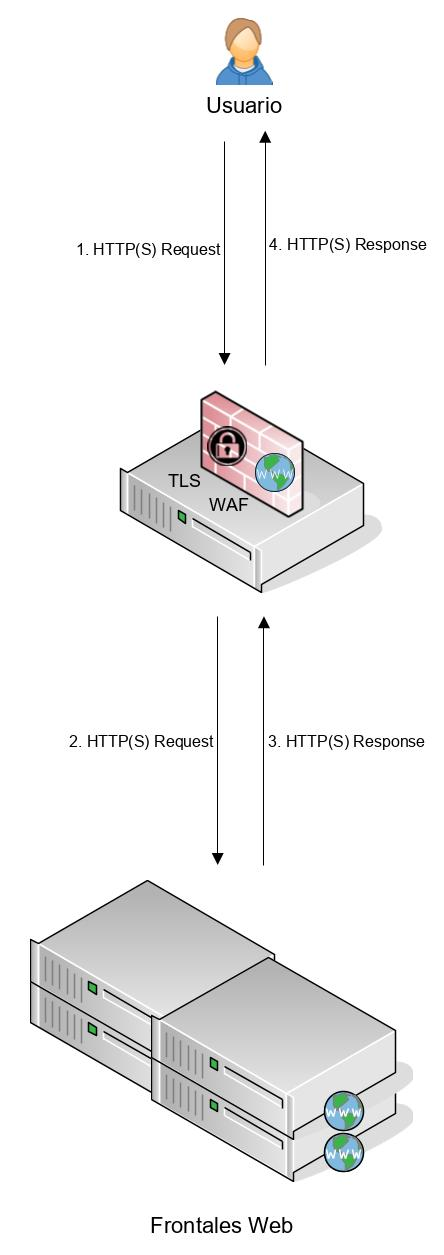
\includegraphics[width=0.4\textwidth]{fig/UseCase1}
        \end{center}
    \end{itemize}
  \item Caso de uso: Petición HTTPS con cifrado punto a punto.
    \begin{itemize}
      \item Actores: Cliente, plataforma web.
      \item Descripción: XXXXXXXX
      \item Diagrama:
        \begin{center}
          \label{fig:CasoUsoXXX}
          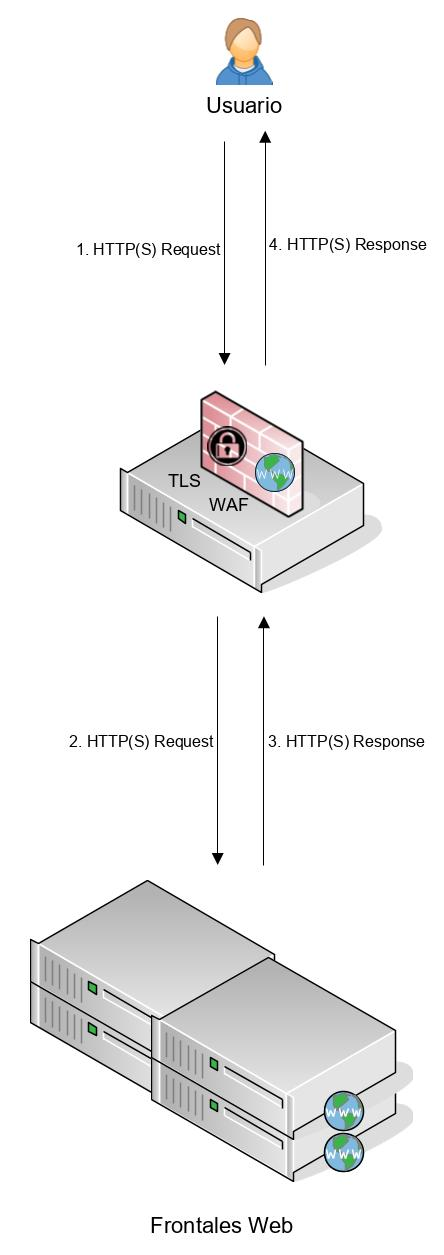
\includegraphics[width=0.4\textwidth]{fig/UseCase1}
        \end{center}
    \end{itemize}
  \item Caso de uso: Petición de validación y firma de certificado TLS a una CA de confianza.
    \begin{itemize}
      \item Actores: \acrlong{CA}.
      \item Descripción: XXXXXXXX
      \item Diagrama:
        \begin{center}
          \label{fig:CasoUsoXXXXX}
          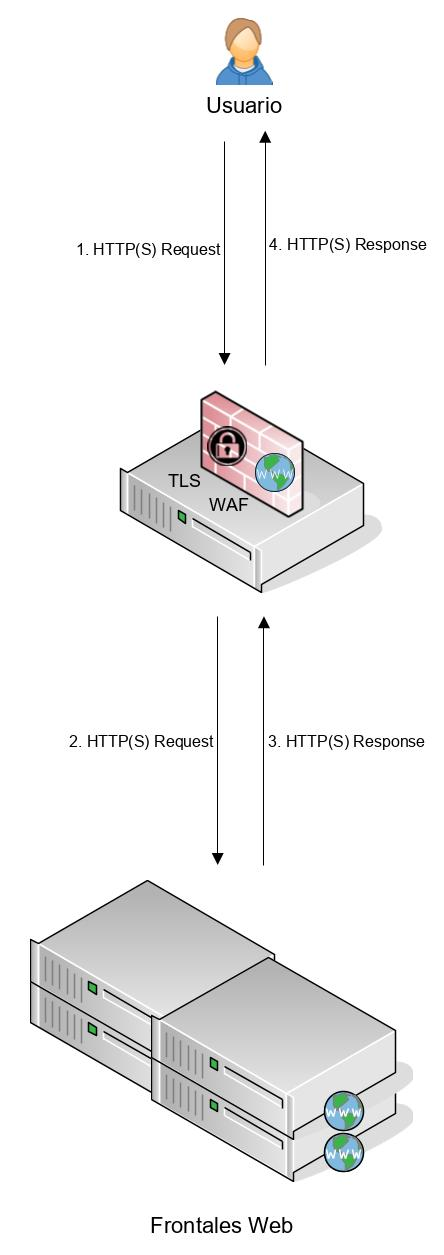
\includegraphics[width=0.4\textwidth]{fig/UseCase1}
        \end{center}
    \end{itemize}
\end{enumerate}


% https://www.gnu.org/licenses/license-compatibility.html
